\documentclass[final]{beamer}

\usepackage{url}
\usepackage[scale=1.2]{beamerposter} % Use the beamerposter package for laying out the poster
\usetheme{confposter} % Use the confposter theme supplied with this template
\setbeamercolor{block title}{fg=ngreen,bg=white} % Colors of the block titles
\setbeamercolor{block body}{fg=black,bg=white} % Colors of the body of blocks
\setbeamercolor{block alerted title}{fg=white,bg=nblue!70} % Colors of the highlighted block titles
\setbeamercolor{block alerted body}{fg=black,bg=dblue!10} % Colors of the body of highlighted blocks
% Many more colors are available for use in beamerthemeconfposter.sty

%-----------------------------------------------------------
% Define the column widths and overall poster size
% To set effective sepwid, onecolwid and twocolwid values, first choose how many columns you want and how much separation you want between columns
% In this template, the separation width chosen is 0.024 of the paper width and a 4-column layout
% onecolwid should therefore be (1-(# of columns+1)*sepwid)/# of columns e.g. (1-(4+1)*0.024)/4 = 0.22
% Set twocolwid to be (2*onecolwid)+sepwid = 0.464
% Set threecolwid to be (3*onecolwid)+2*sepwid = 0.708

\newlength{\sepwid}
\newlength{\onecolwid}
\newlength{\twocolwid}
\newlength{\threecolwid}
\setlength{\paperwidth}{48in} % A0 width: 46.8in
\setlength{\paperheight}{36in} % A0 height: 33.1in
\setlength{\sepwid}{0.024\paperwidth} % Separation width (white space) between columns
\setlength{\onecolwid}{0.22\paperwidth} % Width of one column
\setlength{\twocolwid}{0.464\paperwidth} % Width of two columns
\setlength{\threecolwid}{0.708\paperwidth} % Width of three columns
\setlength{\topmargin}{-0.5in} % Reduce the top margin size
%-----------------------------------------------------------

\usepackage{graphicx}  % Required for including images

\usepackage{booktabs} % Top and bottom rules for tables

%----------------------------------------------------------------------------------------
%	TITLE SECTION 
%----------------------------------------------------------------------------------------

\title{SOEN 6011: SOFTWARE ENGINEERING PROCESSES} % Poster title

\author{Tongwei Zhang ID: 40044711} % Author(s)

\institute{Concordia University: Department of Computer Science and Software Engineering} % Institution(s)

%----------------------------------------------------------------------------------------

\begin{document}

\addtobeamertemplate{block end}{}{\vspace*{2ex}} % White space under blocks
\addtobeamertemplate{block alerted end}{}{\vspace*{2ex}} % White space under highlighted (alert) blocks

\setlength{\belowcaptionskip}{2ex} % White space under figures
\setlength\belowdisplayshortskip{2ex} % White space under equations

\begin{frame}[t] % The whole poster is enclosed in one beamer frame

\begin{columns}[t] % The whole poster consists of three major columns, the second of which is split into two columns twice - the [t] option aligns each column's content to the top

\begin{column}{\sepwid}\end{column} % Empty spacer column

\begin{column}{\onecolwid} % The first column

%----------------------------------------------------------------------------------------
%	OBJECTIVES
%----------------------------------------------------------------------------------------

\begin{alertblock}{ETERNITY: FUNCTIONS }
The project \textbf{ETERNITY: FUNCTIONS} is a medium-sized software engineering project, which is an extension of a typical scientific calculator. The calculator was implements by Java and it was mainly used to process the transcendental function such as $log_b (X)$ and $sinh(x)$. The mainly \textbf{goals} of this project are presented below:
\begin{itemize}
\item Implement the individual function in Java without Java Built-in Math Class.
\item Use the automatic code-review-tool perform a source code review. 
\item Write unit test according to the function requirement.
\item write the function description, requirement description and pseudo-code.
\end{itemize}
\end{alertblock}

%----------------------------------------------------------------------------------------
%	INTRODUCTION
%----------------------------------------------------------------------------------------

\begin{block}{Introduction}
This software engineering project aims to teach us the typical processes of a software engineering project, which contains certain agile methodologies. The transcendental function assigned to me was \textbf{Standard Deviation} $\sigma$, so I needed to write all the related documents and implement this function according to it's formula.
\begin{center}
\begin{equation}
     \sigma=\sqrt{\frac{1}{n}{\sum_{i=1}^n(x_i-\bar{x})^2}}
\end{equation}
\end{center}
\vspace{0.5cm}
However, people usually use n-1 as the denominator to get \textbf{unbiased standard deviation}$^{[1]}$.
\end{block}

%------------------------------------------------
\begin{center}
    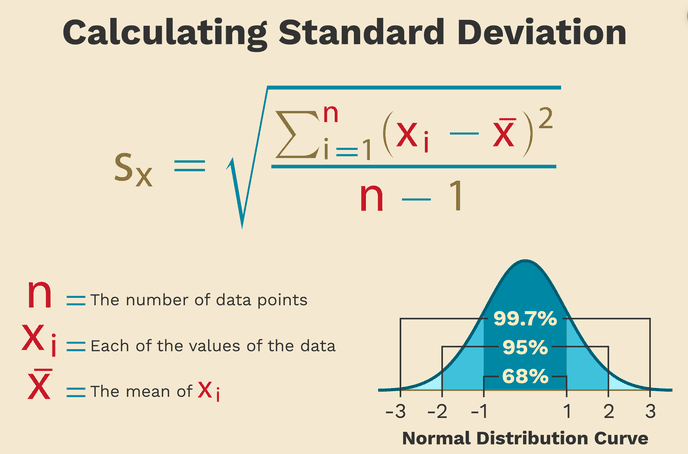
\includegraphics[width=0.8\linewidth]{unbiasedStandardDeviation.png}
\end{center}
%----------------------------------------------------------------------------------------

\end{column} % End of the first column

\begin{column}{\sepwid}\end{column} % Empty spacer column

\begin{column}{\twocolwid} % Begin a column which is two columns wide (column 2)

\begin{columns}[t,totalwidth=\twocolwid] % Split up the two columns wide column

\begin{column}{\onecolwid}\vspace{-.6in} % The first column within column 2 (column 2.1)

%----------------------------------------------------------------------------------------
%	MATERIALS
%----------------------------------------------------------------------------------------

\begin{block}{Software Development process}
The following activities are implemented in the entire development life-cycle.
\begin{itemize}
\item Write the function$(\sigma)$ description to get the sufficient understanding about the function.
\item List the desired requirement that my program should satisfy.
\item Select the suitable algorithms and write the pseudo-code in a uniform format.
\item Implement the Java program.
\item Choice the reasonable approach to launch a source code review.
\item Write the unit test for my function.
\item Test the function from another team member, then judge if all the methods pass the unit test.
\end{itemize}
\end{block}

%----------------------------------------------------------------------------------------

\end{column} % End of column 2.1

\begin{column}{\onecolwid}\vspace{-.6in} % The second column within column 2 (column 2.2)

%----------------------------------------------------------------------------------------
%	METHODS
%----------------------------------------------------------------------------------------

\begin{block}{Methods}

According the formula above, I have to calculate the average value according to the input parameters. Then calculate the sum of square of sample value subtract average value. Then divided by the number of samples subtract 1 to correct the bias. The \textbf{key step} is calculate the \textbf{Arithmetic square root}. I have to use the mathematical approach since this method is more accurate and it can control the decimal digit number. The method I used is called \textbf{Newton-Raphson method}, it used tangent is the linear approximation of the curve
to get the result.
\vspace{0.5cm}
\begin{center}
    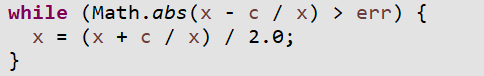
\includegraphics[width=0.8\linewidth]{keyProcess.png}
\end{center}
Key process of Newton-Raphson method.
\end{block}

%----------------------------------------------------------------------------------------

\end{column} % End of column 2.2

\end{columns} % End of the split of column 2 - any content after this will now take up 2 columns width

%----------------------------------------------------------------------------------------
%	IMPORTANT RESULT
%----------------------------------------------------------------------------------------

\begin{alertblock}{Accuracy of result}

Via the method above and the unit test, We can know this method can get the as same result of standard deviation as the scientific calculator result.

\end{alertblock} 

%----------------------------------------------------------------------------------------

\begin{columns}[t,totalwidth=\twocolwid] % Split up the two columns wide column again

\begin{column}{\onecolwid} % The first column within column 2 (column 2.1)
\vspace{-2cm}
\begin{block}{Functions Display}
For the convenience of users, I designed the textual interface to show the prompt message and error reminder:
\begin{center}
    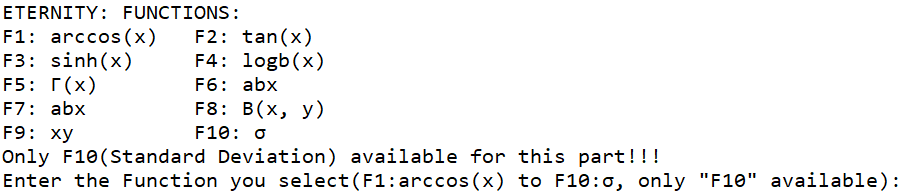
\includegraphics[width=1\linewidth]{interface1.png}
\end{center}
The function selection interface, only F10 available in this part.
\begin{center}
    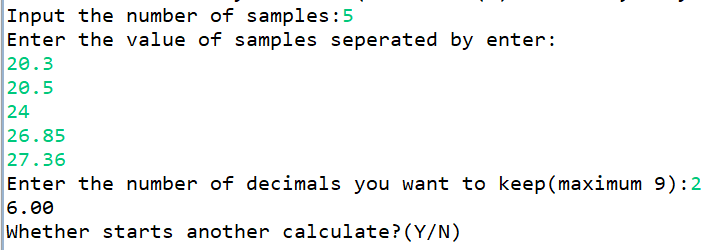
\includegraphics[width=1\linewidth]{interface2.png}
\end{center}
\vspace{-0.7cm}
Input the needed parameter then get the result.
\vspace{-1cm}
\begin{center}
    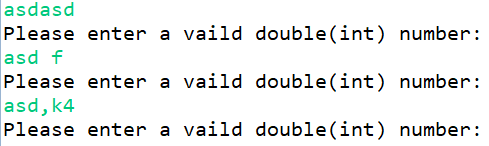
\includegraphics[height=0.2\linewidth,width=1\linewidth]{error1.png}
\end{center}
\end{block}

%----------------------------------------------------------------------------------------

\end{column} % End of column 2.1

\begin{column}{\onecolwid} % The second column within column 2 (column 2.2)

%----------------------------------------------------------------------------------------
%	RESULTS
%----------------------------------------------------------------------------------------
\vspace{-2cm}
\begin{block}{Learnt from code review}
According to the source code review from my teammate, I realized several problems in my source code.
\vspace{-2cm}
\begin{itemize}
\item One of the method contains high complexity.
\item When the program implements the String compare statement, Make sure the string that is not empty should be placed in front. Otherwise, it will exist the possibility of NullPointerException.
\end{itemize}
From the review result, we can know several things that we ignore normally. It also prove that the automatic code review tool is convenience to check the detail problem of the source code. This project even just a medium-size software project. On the other hand, high complexity means this method has a high branch. It means that this part is hard to maintain and modify. Since it will introduce the new bugs at most of time. Furthermore, we have to notice the detail convention like put the nun-empty string at the front of \textbf{equals()} method. It reduces the chance of an running exception happened and  can guarantee the application works well in a long-term in some extend.

\end{block}

%----------------------------------------------------------------------------------------

\end{column} % End of column 2.2

\end{columns} % End of the split of column 2

\end{column} % End of the second column

\begin{column}{\sepwid}\end{column} % Empty spacer column

\begin{column}{\onecolwid} % The third column

%----------------------------------------------------------------------------------------
%	CONCLUSION
%----------------------------------------------------------------------------------------

\begin{block}{Learnt from testing}

According to the feedback from my teammate, I noticed that all the Junit test passed. However, the problem is the \textbf{test case ID} is not very clear. It is not a big problem in this small size project. But if it happened in a large-scale project, that is a serious problem. Without the clear traceable ID, the developer and tester cannot work \textbf{collaboratively efficiency}. It will increase the development lifcycle, cause the delay of product. The developer also cannot find where the problem is. From the testing feedback, I learnt that we not only need to ensure the functional requirement are satisfied, but also to keep the long-term maintenance.

\end{block}

%----------------------------------------------------------------------------------------
%	ADDITIONAL INFORMATION
%----------------------------------------------------------------------------------------

\begin{block}{Additional Information}

In the process of writing the Junit test, I used the \textbf{assertEquals} method to check the correctness of method \textbf{isDouble()}. One interesting is, in order to test the expected value and real value from method, I have to set a deviation. If the difference between expected value and real value within this deviation, the assertEquals will get the true result. This phenomenon is caused by the Double value is just a approximation of real value.

\end{block}

%----------------------------------------------------------------------------------------
%	REFERENCES
%----------------------------------------------------------------------------------------

\begin{block}{References}

$\left[1\right]$ \url{https://en.wikipedia.org/wiki/Unbiased_estimation_of_standard_deviation} \\
$\left[2\right]$ \url{http://www.latextemplates.com/template/jacobs-landscape-poster}

\end{block}

%----------------------------------------------------------------------------------------
%	CONTACT INFORMATION
%----------------------------------------------------------------------------------------

\setbeamercolor{block alerted title}{fg=black,bg=norange} % Change the alert block title colors
\setbeamercolor{block alerted body}{fg=black,bg=white} % Change the alert block body colors

\begin{alertblock}{Remarks}

\begin{itemize}
\item Github: \href{https://github.com/Alex44711}{https://github.com/Alex44711}
\end{itemize}

\end{alertblock}

\begin{center}
\begin{tabular}{ccc}

\includegraphics[width=0.4\linewidth]{encs.png} & \hfill & 
\includegraphics[width=0.4\linewidth]{encs.png}
\end{tabular}
\end{center}

%----------------------------------------------------------------------------------------

\end{column} % End of the third column

\end{columns} % End of all the columns in the poster

\end{frame} % End of the enclosing frame

\end{document}
